Various experiments were conducted to find the way to implement functions mentioned in section 3: device discovery, whitelist extraction, network filtering. Next, we would like to explain IoT system used as the test subject in this experiment, also the elaborate detail for each experiment.

\section{IoT system}
\subsection{eroom}
\subsection{10F}

\section{Packet Capturing}
\subsection{Purpose}
Packet data is captured, then analyzed to investigate the pattern of IoT system communication. This packet data capturing method is used in both “Device discovery experiment”, and “Whitelist extraction” 

\begin{figure}[h]
    \centering 
    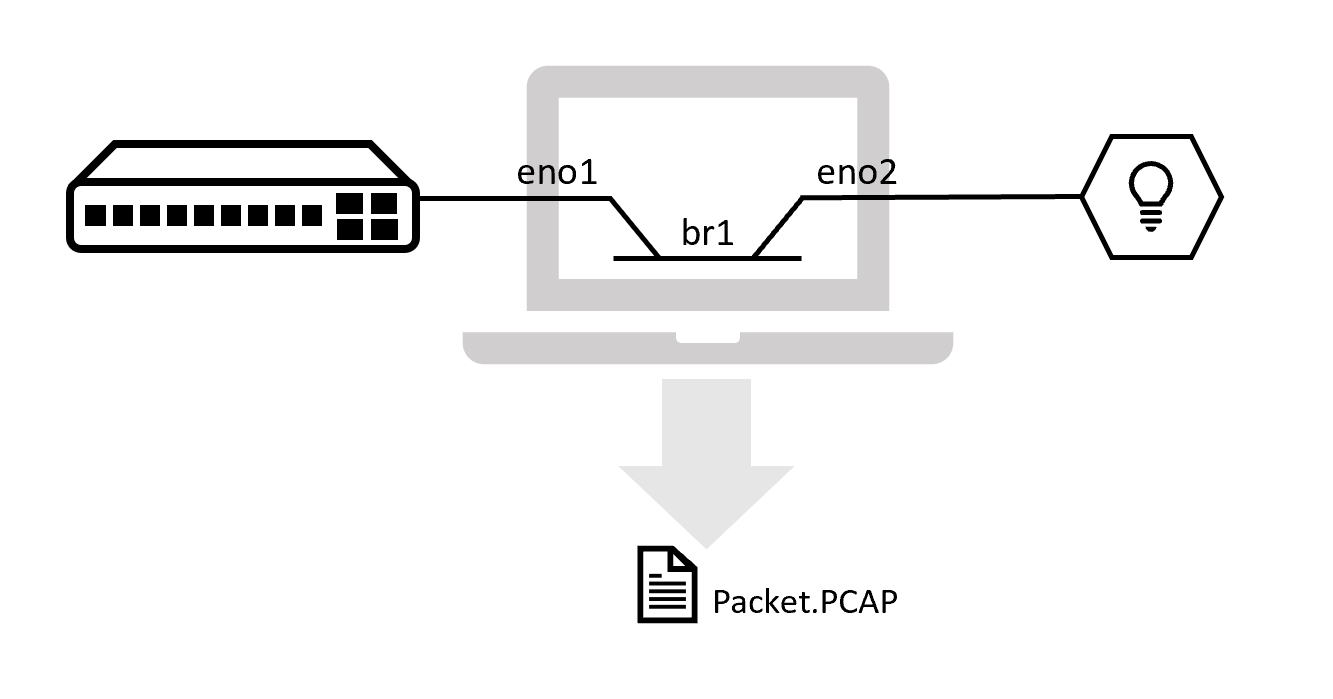
\includegraphics[width=0.6\textwidth]{4_packet_capturing}
    \caption{Packet Capturing}
    \label{fig:s4_packet_capturing}
\end{figure}

\subsection{Method}
First, we inserted a computer in between Switch and any IoT devices, we aim to capture its packet. As a requirement, computer used in this procedure must has at least 2 network interfaces. One network interface was connected to the switch, while another was connected to IoT device (Figure \ref{fig:s4_packet_capturing}). After that, we created network bridge to connect two of inserted computer network interfaces. Any computers run with Linux kernel can initiate a bridge using “brctl” command. Then packet would be captured using tpcdump command. (tcpdump is a TCP/IP packet sniffing command) Collected data was saved into PCAP format. 

\subsection{Result}
Packet Description

\section{Device Discovery}
\subsection{Purpose}
Device discovery is a process conducted to find all devices in LAN. Their IP address and MAC address is necessary when performing whitelist extraction.  

\subsection{Method}
In this experiment, we had tested capturing devices’ packet in three patterns: pattern A and B. In pattern A (Figure \ref{fig:s4_pattern_a}), we created a computer bridge between all devices and switch, while in pattern B (Figure \ref{fig:s4_pattern_b}), we connected PC to one of IoT devices switch’s ports, and capturing packet coming through. The gathered packet is then analyzed to find list of hosts in LAN.  

\begin{figure}
    \centering
    \begin{subfigure}[b]{0.35\textwidth}
        \centering
        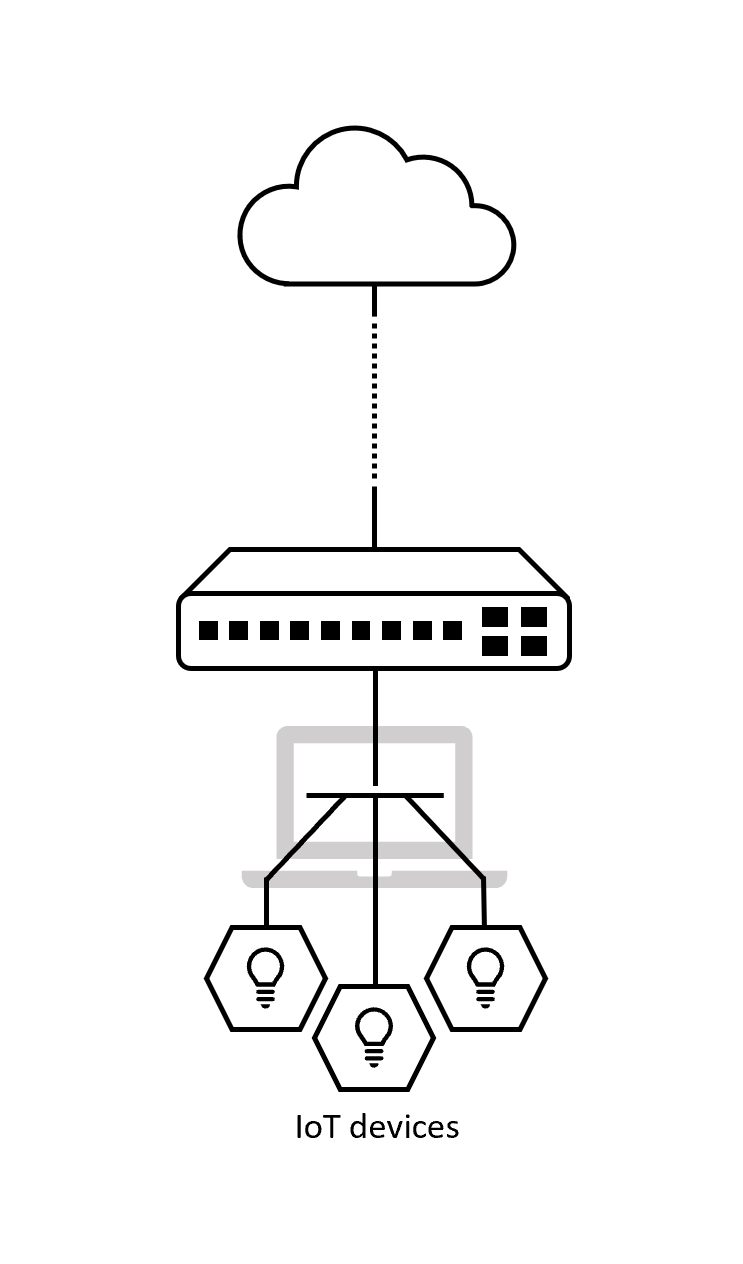
\includegraphics[width=\textwidth]{4_pattern_a}
        \caption{Pattern A : Capturing packet from bridge PC between all devices and switch}
        \label{fig:s4_pattern_a}
    \end{subfigure}
    \hspace{1.5cm}
    \begin{subfigure}[b]{0.35\textwidth}
        \centering
        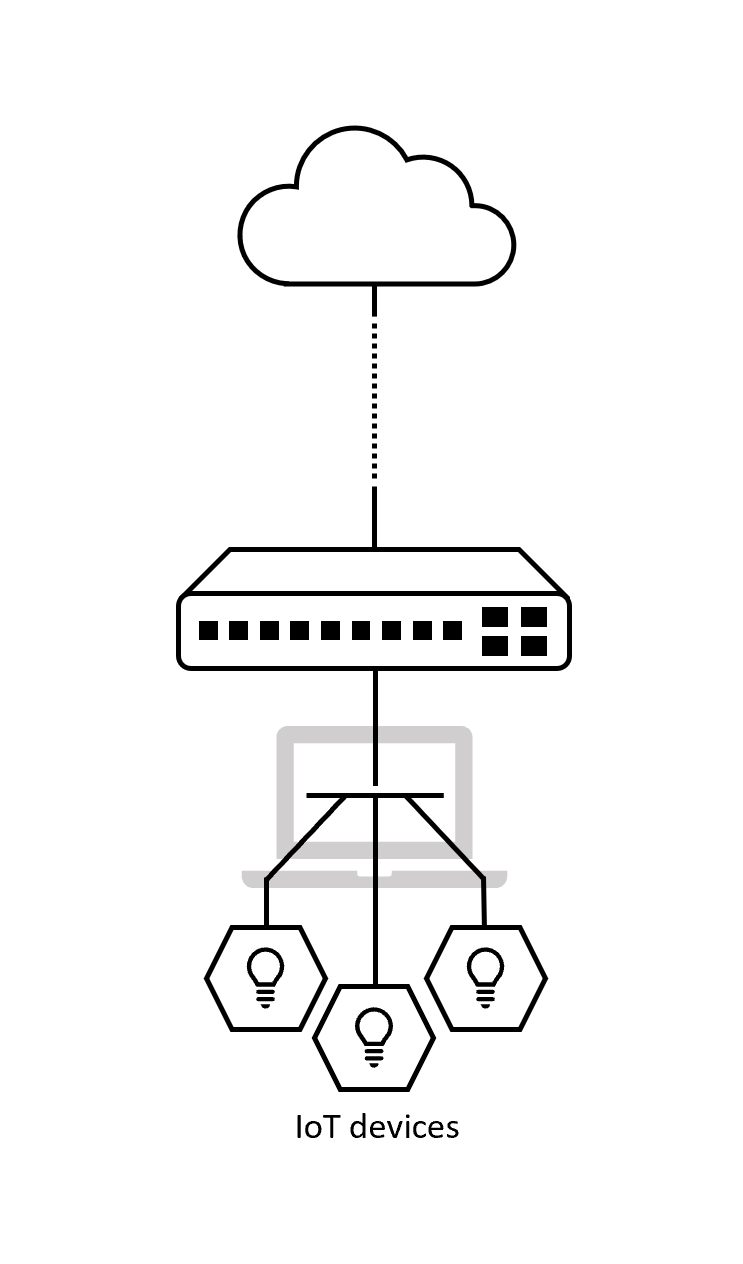
\includegraphics[width=\textwidth]{4_pattern_a}
        \caption{Pattern B : Capturing packet from PC connected to one of switch port}
        \label{fig:s4_pattern_b}
    \end{subfigure} 
    \caption{Packet Capturing Patterns}
    \label{fig:s4_packet_pattern}
\end{figure}

In this experiment, we have tested host detection algorithm constructed with three approaches: Detecting hosts by ARP request, by ARP reply and by gratuitous ARP. 

\begin{itemize}
    \item \textbf{ARP request} is Arp packet with opcode equal to 1 and Target MAC address equal to “00:00:00:00:00:00”. We considered Sender of this packet to be host in LAN and added tuple of its MAC address (SHA) and IP address (SPA) to host list.
    \item \textbf{ARP reply} is Arp packet with opcode equal to 2. We added both Target and Sender of this packet to host list. 
    \item \textbf{Gratuitous ARP} is Arp packet which has is sender IP address equal to target IP address, its opcode equal to 1, and has target MAC address equal to “00:00:00:00:00:00”. We added Sender of this packet it to host list.  
\end{itemize}

We tested our approaches in the following combination.

\begin{table}[]
    \centering \begin{tabular}{l|ccc}
        &  ARP request  & ARP reply & Gratuitous ARP  \\ \hline
        Pattern A  &  $\bigcirc$ & - & $\bigcirc$  \\
        Pattern B  &  - & $\bigcirc$ & $\bigcirc$  
    \end{tabular}
    \caption{Tested Pattern}
    \label{table:s4_patterns}
\end{table}

\subsection{Result}
\subsection{Discussion}


\section{Whitelist Extraction}
\subsection{Purpose}
In order to secure our IoT system, the suitable whitelist for each device is crucial. By implementing whitelist, not only can we guarantee that system can withstand the attacks from outside, but we can also prevent our infected device from attacking other servers. In this experiment, we want to find an algorithm to extract the secure hosts. 

\begin{figure}[h]
    \centering 
    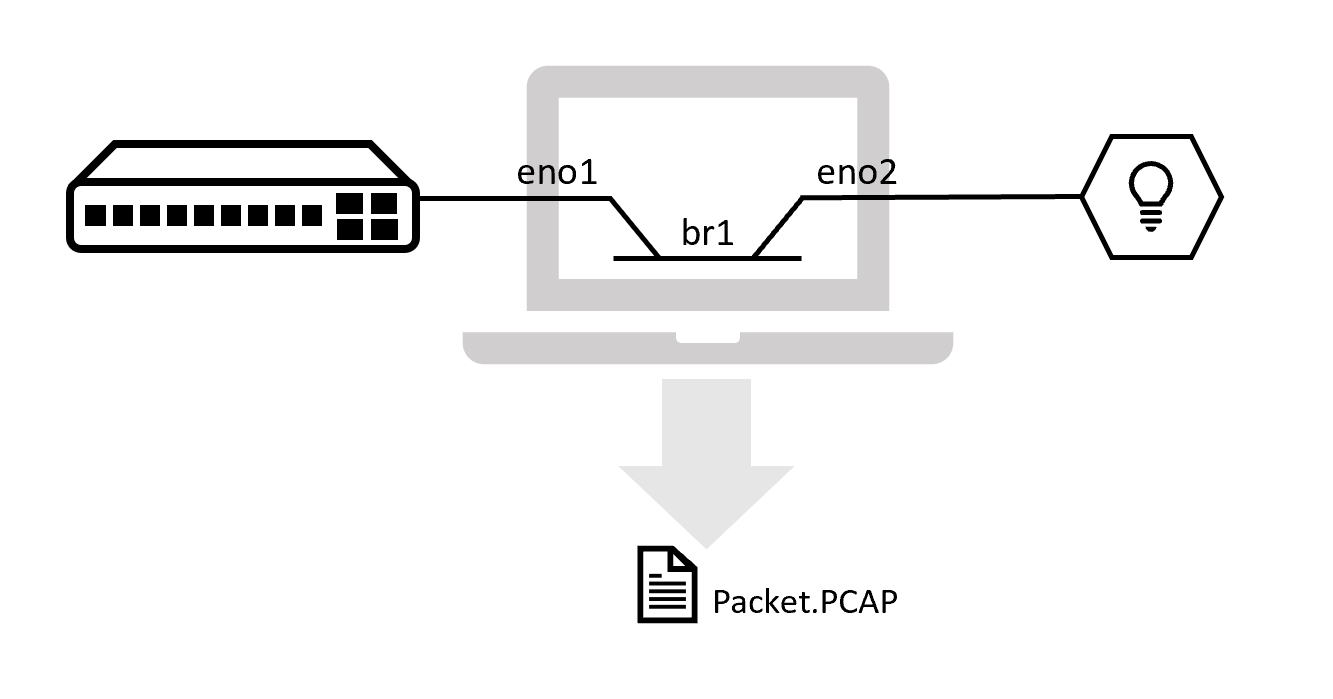
\includegraphics[width=0.6\textwidth]{4_packet_capturing}
    \caption{Packet Capturing}
    \label{fig:s4_packet_capturing}
\end{figure}

\subsection{Method}
\paragraph{Program and Algorithm}
We wrote program to extract whitelist for each device extracted in Device Discovery, using collected traffic packet as an input. Next, we would like to explain how program works.

\begin{enumerate}
    \item Program take network traffic data as an input. 
    \item Traffic data was divided into a smaller group of time $\tau$. Only IP packet with TCP/UDP as its transmission protocol was considered. 
    \item In each group, we looked at each host’s first interaction (packet) with edge device.
    \begin{itemize}
        \item If packet is originated from device, we decide that this host might be secure.
        \item If packet is destined to device, we decide that this host might be insecure.
    \end{itemize}
    \item If in most group (90\%), host that communicated with device was identified as “might be secure”, we add it to device’s whitelist.
    \item The output of program is devices’ whitelist saving in JSON format.
\end{enumerate}

\subsection{Result}
\subsection{Discussion}

\section{Packet Filtering}
\subsection{Purpose}
After whitelist has been extracted, we can keep the network traffic of IoT system secure by filtering unwanted traffic.  

\subsection{Method} 
 
In this experiment, we created a filter by combining 
\colorbox{white}{\lstinline[basicstyle=\ttfamily\color{black}]|iptables|} and 
\colorbox{white}{\lstinline[basicstyle=\ttfamily\color{black}]|NetfilterQueue-python|}. 
\colorbox{white}{\lstinline[basicstyle=\ttfamily\color{black}]|iptables|} is a Linux command that allows user to filter network packets by configure tables of IP packet filter rules in the Linux kernel. We wrote a program that take the JSON output of whitelist extraction program as an input a create an 
\colorbox{white}{\lstinline[basicstyle=\ttfamily\color{black}]|iptables|}
iptables script as its output. Next is the template of our script.
\\

\lstset{
  breaklines = true,
  classoffset=1,
  frame=tRBl,
  framesep=5pt,
  showstringspaces=false,
  numbers=left,
  stepnumber=1,
  tabsize=2,
}


\begin{lstlisting}[label=sh]
# iptables -F  
# iptables -P FORWARD DROP 
# iptables -A FORWARD -p [udp|tcp] -dport [port number] -d [device secure host IP] -s [device ip] -j ACCEPT 
# iptables -A FORWARD -p [udp|tcp] -dport [port number] -d [device ip] -s [device secure host IP] -j ACCEPT
\end{lstlisting}

\begin{itemize}
    \item 1st line, -F command is to clean the exist rule in iptables. 
    \item 2nd line states that our default policy for any packet FORWARD through is computer is DROP 
    \item 3rd and 4th line states that only device’s hosts with specific protocol, port number can communicate with the device.
\end{itemize}

\begin{figure}[h]
    \centering 
    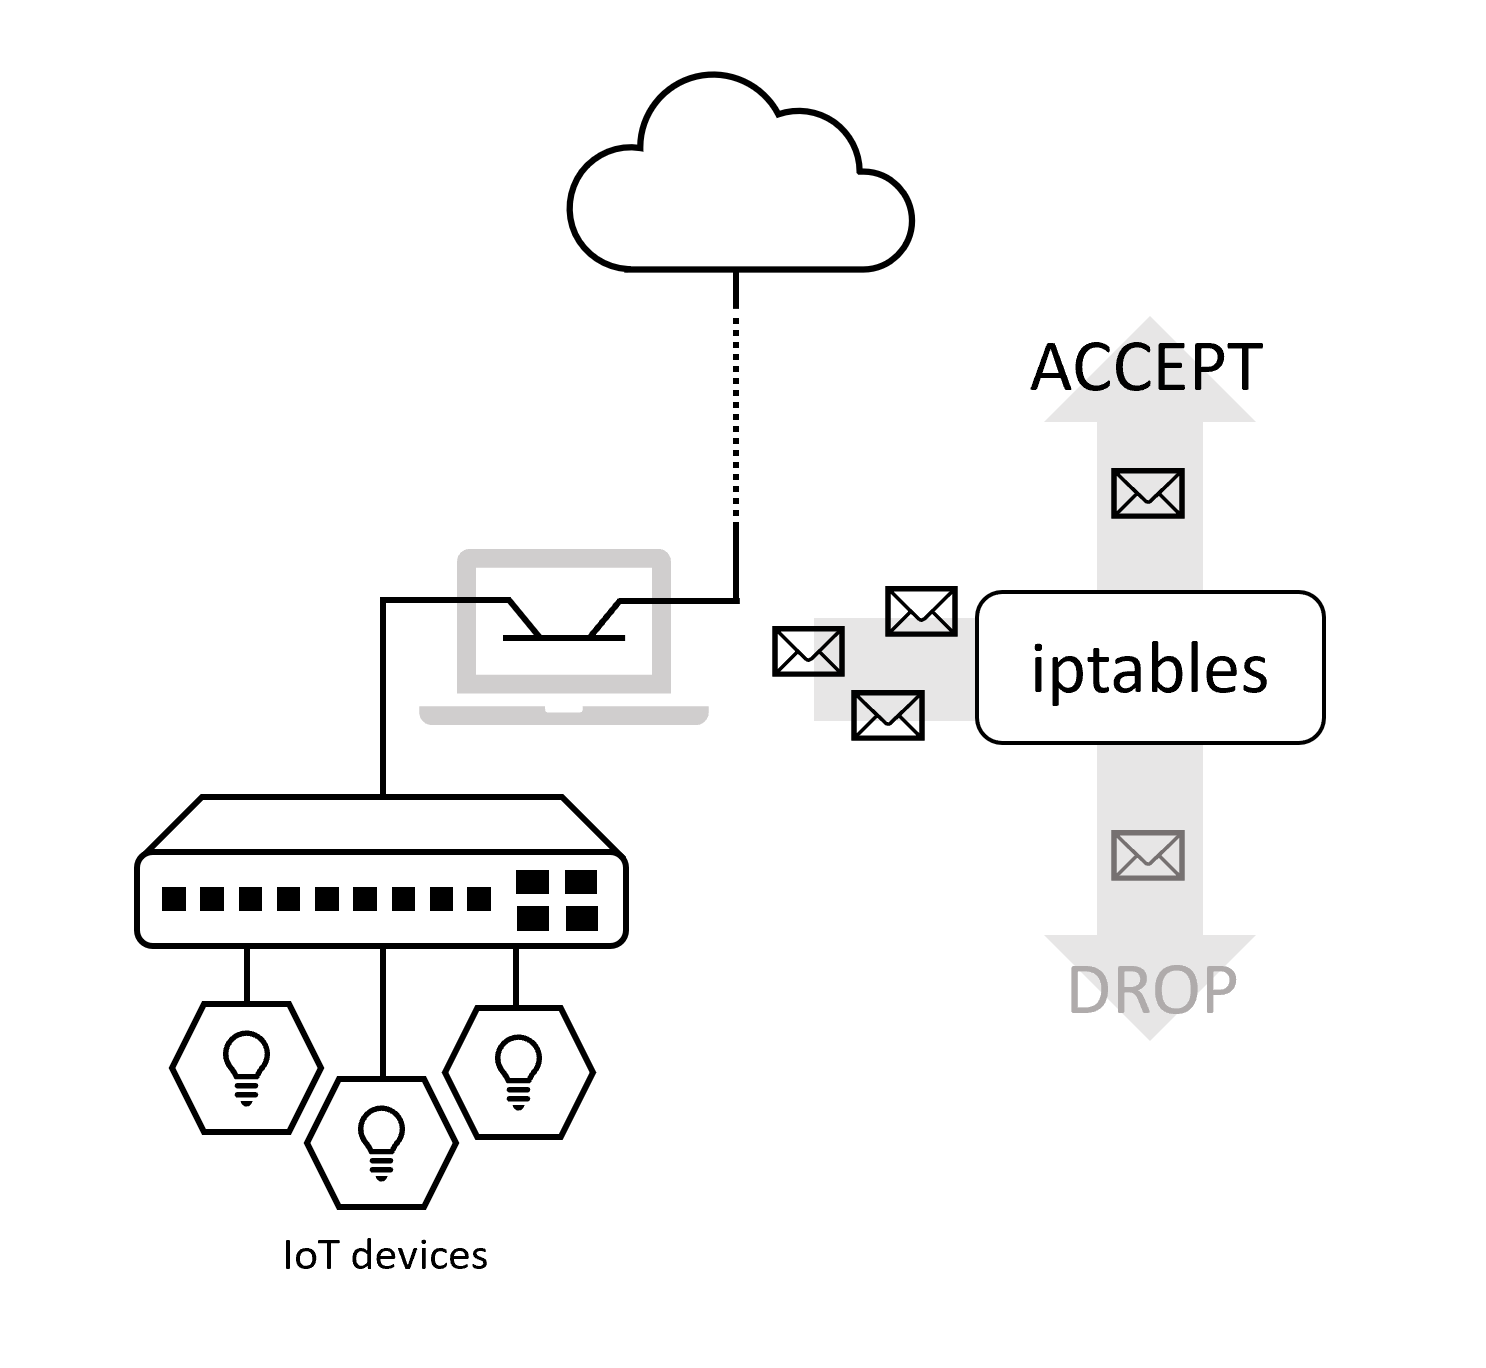
\includegraphics[width=0.6\textwidth]{4_filter}
    \caption{Packet Filtering using iptables}
    \label{fig:s4_filter}
\end{figure} 

Then we ran this script on computer bridging between the internet and the switch, or the switch and devices (Figure \ref{fig:s4_filter}). This allowed us to filter all unnecessary packets and kept our IoT system secure. 
Next step, we wanted to evaluate the performance of our whitelist. Therefore, instead of dropping and accepting at the iptables, we configured iptables to pass all dropped packets to our “NetfilterQueue” python program. NetfilterQueue is a module that provides access to packets matched by iptables rule, we can analyze those packets using “kamene” (also known as “scapy”).

\begin{figure}[h]
    \centering 
    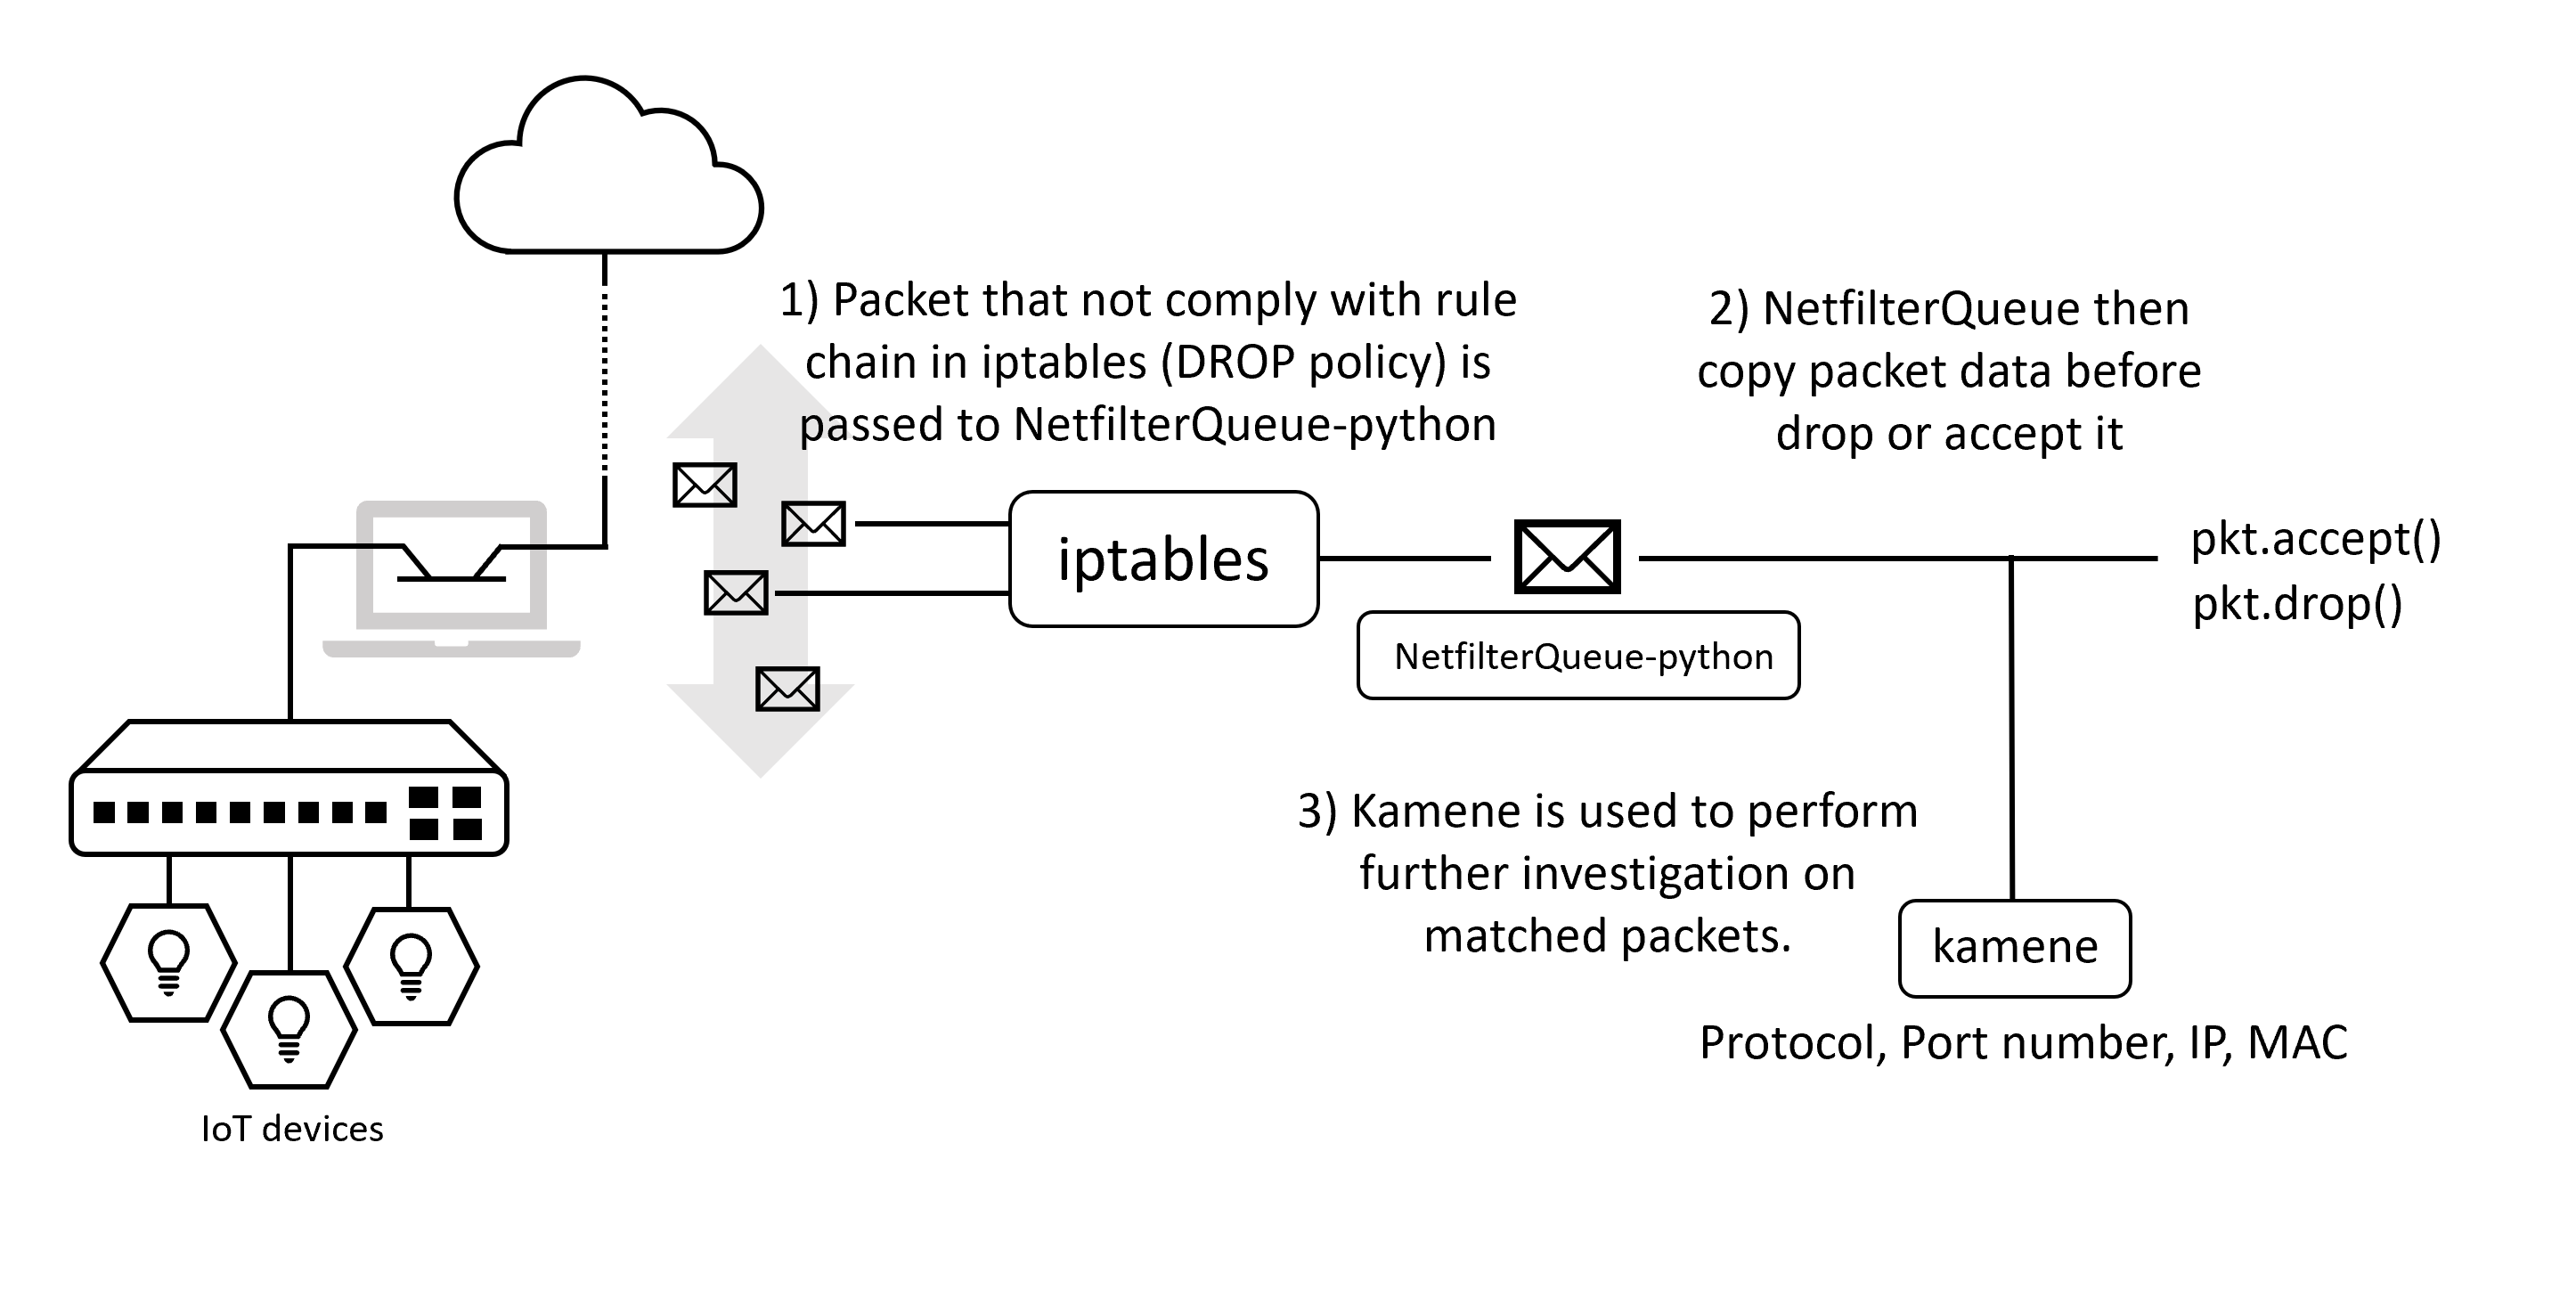
\includegraphics[width=\textwidth]{4_netfilter} 
    \caption{Analyzing matched packet by iptables using NetfilterQueue-python module and kamene}
    \label{fig:s4_netfilter}
\end{figure} 